\chapter{Experimental Setup}

This chapter presents the experimental setup used to evaluate the task-
priority control framework developed in this thesis. It begins with an 
overview of the Eelume robot, including its mechanical structure, sensor suite
, communication systems, and suitability for underwater manipulation tasks. 
Following that, the software tools and interfaces used to control the robot 
and simulate its behavior are described. The chapter also outlines key 
assumptions and limitations in the experimental environment, including sensor 
noise and system constraints. Finally, the experimental procedures are detailed
, describing how specific robot behaviors will be tested and what kinds of 
responses are expected. Together, these sections provide the necessary context 
for understanding the practical validation of the proposed control approach.

% -----------------------------------------------------------------------------
\section{The Eelume Robot}

The Eelume \(500\) model M robot is a snake-like underwater vehicle developed by 
the company Eelume AS. It is designed for subsea inspection and light 
intervention tasks, and can be deployed in a variety of environments, 
including offshore wind farms, fish farms, and oil and gas installations. The 
system is highly modular, enabling a wide range of use cases.
The robot can operate either as an \gls{auv}, using an acoustic communication 
link, or as an \gls{rov} via a fiber-optic tether. A computer rendering of the 
Eelume robot is shown in \autoref{fig:eelume:stopdown}.

\begin{figure}[h!]
    \centering
    \includegraphics[width=\textwidth]{assets/ignored/s-topdown.png}
    \caption{A computer rendering of the Eelume robot configured in an S-shape.}
    \label{fig:eelume:stopdown}
\end{figure}

The Eelume robot can be equipped with a wide range of sensors, including a \gls{dvl},
\gls{imu}, \gls{uhi}, sonar, echo-sounder, fluorometer, \gls{ct}, and 
cameras. It uses an onboard Sunstone \gls{ins} from Kongsberg for navigation, supported by the \gls{dvl}
and an acoustic positioning system. At the surface, it is equipped with an 
antenna for satellite communication via Iridium, as well as \gls{gps}. Ballast 
modules allow for buoyancy control, enabling the robot to remain slightly 
positively buoyant in both fresh and salt water, depending on the configuration.
The onboard battery supports up to $8$ hours of operation, depending on 
usage and setup.

The configuration used in the experiments described in this thesis is similar 
to that shown in \autoref{fig:eelume:stopdown}, with some changes to module 
arrangement. The front of the robot is equipped with a \gls{uhi} instead of 
the forward-looking sonar shown in the figure. The overall shape, including 
thruster and joint placement, remains close to what is depicted. In this 
configuration, the Eelume robot weighs approximately $190$ kg and measures 
about $6.05$ m in length. From left to right in the image, we define the three 
links as \textit{tail}, \textit{body}, and \textit{head}, respectively. The 
following $5$ coordinate frames are attached to the robot:
\begin{itemize}
\item \textbf{tail} – the very end of the tail link, located on the left in \autoref{fig:eelume:stopdown}.
\item \textbf{tail center} – the center of the tail link.
\item \textbf{body} – the center of the body link.
\item \textbf{head center} – the center of the head link.
\item \textbf{head} – the very end of the head link, located on the right in \autoref{fig:eelume:stopdown}.
\end{itemize}

The $x$-axes of these frames align with the robot, pointing "forward." The $z$-
axes point downward toward the shadow, which also corresponds to the downward 
direction in \autoref{fig:eelume:stopdown}. The $y$-axes are defined by the 
right-hand rule. As the robot moves, the frames remain attached to their 
respective links and rotate with them. The coordinate frames at the centers of 
the head and tail links are useful for defining hydrodynamic damping forces, 
while the remaining three frames are primarily used for task definitions.
\begin{figure}[h!]
    \centering
    \begin{subfigure}{0.45\textwidth}
        \centering
        \includegraphics[width=\textwidth]{assets/ignored/s-1.png}
        \caption{The Eelume robot bending joints \(2\) and \(4\) about the $z$-axis.}
        \label{fig:eelume:joints:1}
    \end{subfigure}
    \hfill
    \begin{subfigure}{0.45\textwidth}
        \centering
        \includegraphics[width=\textwidth]{assets/ignored/s-2.png}
        \caption{The Eelume robot bending joints \(1\) and \(3\) about the $y$-axis.}
        \label{fig:eelume:joints:2}
    \end{subfigure}
    \caption{The Eelume robot with its two joints shown in different configurations.}
\label{fig:eelume:joints}
\end{figure}
The three links are connected by two joints, each with two degrees of freedom—
allowing rotation about both the $y$ and $z$ axes. We number the individual joints from
\(1\) to \(4\), indicating its location along the robot; joint \(1\) is
the closest to the head while joint \(4\) is the closest to the tail.
\autoref{fig:eelume:joints} illustrates the joints in two different rotational configurations. The robot 
features two sets of $4$ thrusters: one set on the tail and another on the 
body link near the head joint. Each thruster can be independently controlled 
and provides bidirectional thrust. The thruster arrangement is shown in
\autoref{fig:eelume:thrusters}. When the robot is in a straight configuration, 
forces and moments can be generated independently in all $6$ \gls{dof}s. 
Together with the $2 \times 2$ \gls{dof}s from the joints, this results in a 
total of $10$ \gls{dof}s for this Eelume configuration. The joints are 
actuated by motors, bringing the total number of independent inputs to $12$:
$8$ thrusters and $4$ joint actuators. Some key parameters of the Eelume robot
are summarized in \autoref{tab:eelume:keynumbers}.
\begin{table}[h]
    \centering
    \begin{tabular}{|c|c|c|}
        \hline
        Parameter  & Value & Unit   \\ \hline \hline
        Total length & 6.05 & m     \\ \hline
        Total weight & 190  & kg    \\ \hline
        Diameter & 20 & cm    \\ \hline
        Joint length & x & cm    \\ \hline
        Length head link & x & m     \\ \hline
        Length body link & x & m     \\ \hline
        Length tail link & x & m     \\ \hline
        Weight head link & x & kg     \\ \hline
        Weight body link & x & kg     \\ \hline
        Weight tail link & x & kg     \\ \hline
        Maximum thruster wattage & \(125\) & W     \\ \hline
        Maximum joint torque & \(16\) & Nm     \\ \hline
        \hline
    \end{tabular}
    \caption{Key parameters of the Eelume robot.}
    \label{tab:eelume:keynumbers}
\end{table}
The Eelume robot is an excellent platform for testing task-priority controllers.
This is largely due to its high number of \gls{dof}s, allowing for the 
execution of multiple tasks before kinematic constrains limit the robot. Additionally, 
the robot is highly coupled—motion in one link induces forces and moments in 
others. Task-priority control is an elegant approach for managing this coupling
, as the controller architecture inherently accommodates such interactions. In 
contrast, a typical large \gls{rov} with a manipulator arm exhibits minimal 
coupling, allowing the arm and vehicle to be controlled separately. In this 
respect, the Eelume robot is unique: it combines high \gls{dof} count with 
strong coupling, making it a compelling testbed for task-priority control.

% -----------------------------------------------------------------------------
\section{Tools and software}

The Eelume robot is controlled using a low-level \gls{api} that Eelume AS made
available in the beginning of 2025. This api provides access to low-level methods
for controlling the robot's thrusters and joints, as well as for reading sensor
data, and \gls{ins} measurements. The \gls{api} is implemented in C/C++ and communicates with the robot over
an ethernet connection. Because the \gls{api} is low-level, a lot of code had
to be written to implement the task-priority control framework, everyting from
lower-level controllers, task definitions, and kinematics. The collection of
code used to control the Eelume robot is created as a standalone C++ library
and is refered to as \gls{eck}.

The control kit is designed to be modular, allowing for easy integration of
new tasks and controllers. The library provides a set of virtual base classes,
one for a controller and one for a connection to the Eelume robot, along with
a set of concrete implementations for these classes. Setting and reading data
from the robot is done through the \gls{api} using a connection class, while 
a simulator is also provided for testing the controllers without the need for
a physical robot. Lower level \gls{dp} controllers, as well as higher-level
task-priority controllers are also implemented.

The simulator is designed to mimic the behavior of the Eelume robot as closely
as possible, without much time spent on modeling the hydrodynamics and coupling
between the links. The kinematics of the robot is tought to be accurately
implemented. Because of the virtual base classes, the real robot can be used
interchangeably without recompiling the code. This allows for easy testing of
the controllers after veryfing that they work in the simulator.

In addition to the control kit, the need for vizualization of the robot and
the tasks was identified. A simple visualizer was created to display the robot
in real time as experiments are conducted. The visualizer is implemented in
C++ using the OpenGL graphics library. The control kit communicates with the
visualizer over \gls{udp} sockets, sending the robot's state and task definitions.
Eelume robot that are presented in this thesis are created using this visualizer.
An example of the visualizer as it is used during experiments is shown in
\autoref{fig:eelume:visualizer}. One can see gridlines in the background, and
an axis system in the center showing the \gls{ned} frame origin.
\begin{figure}[h!]
    \centering
    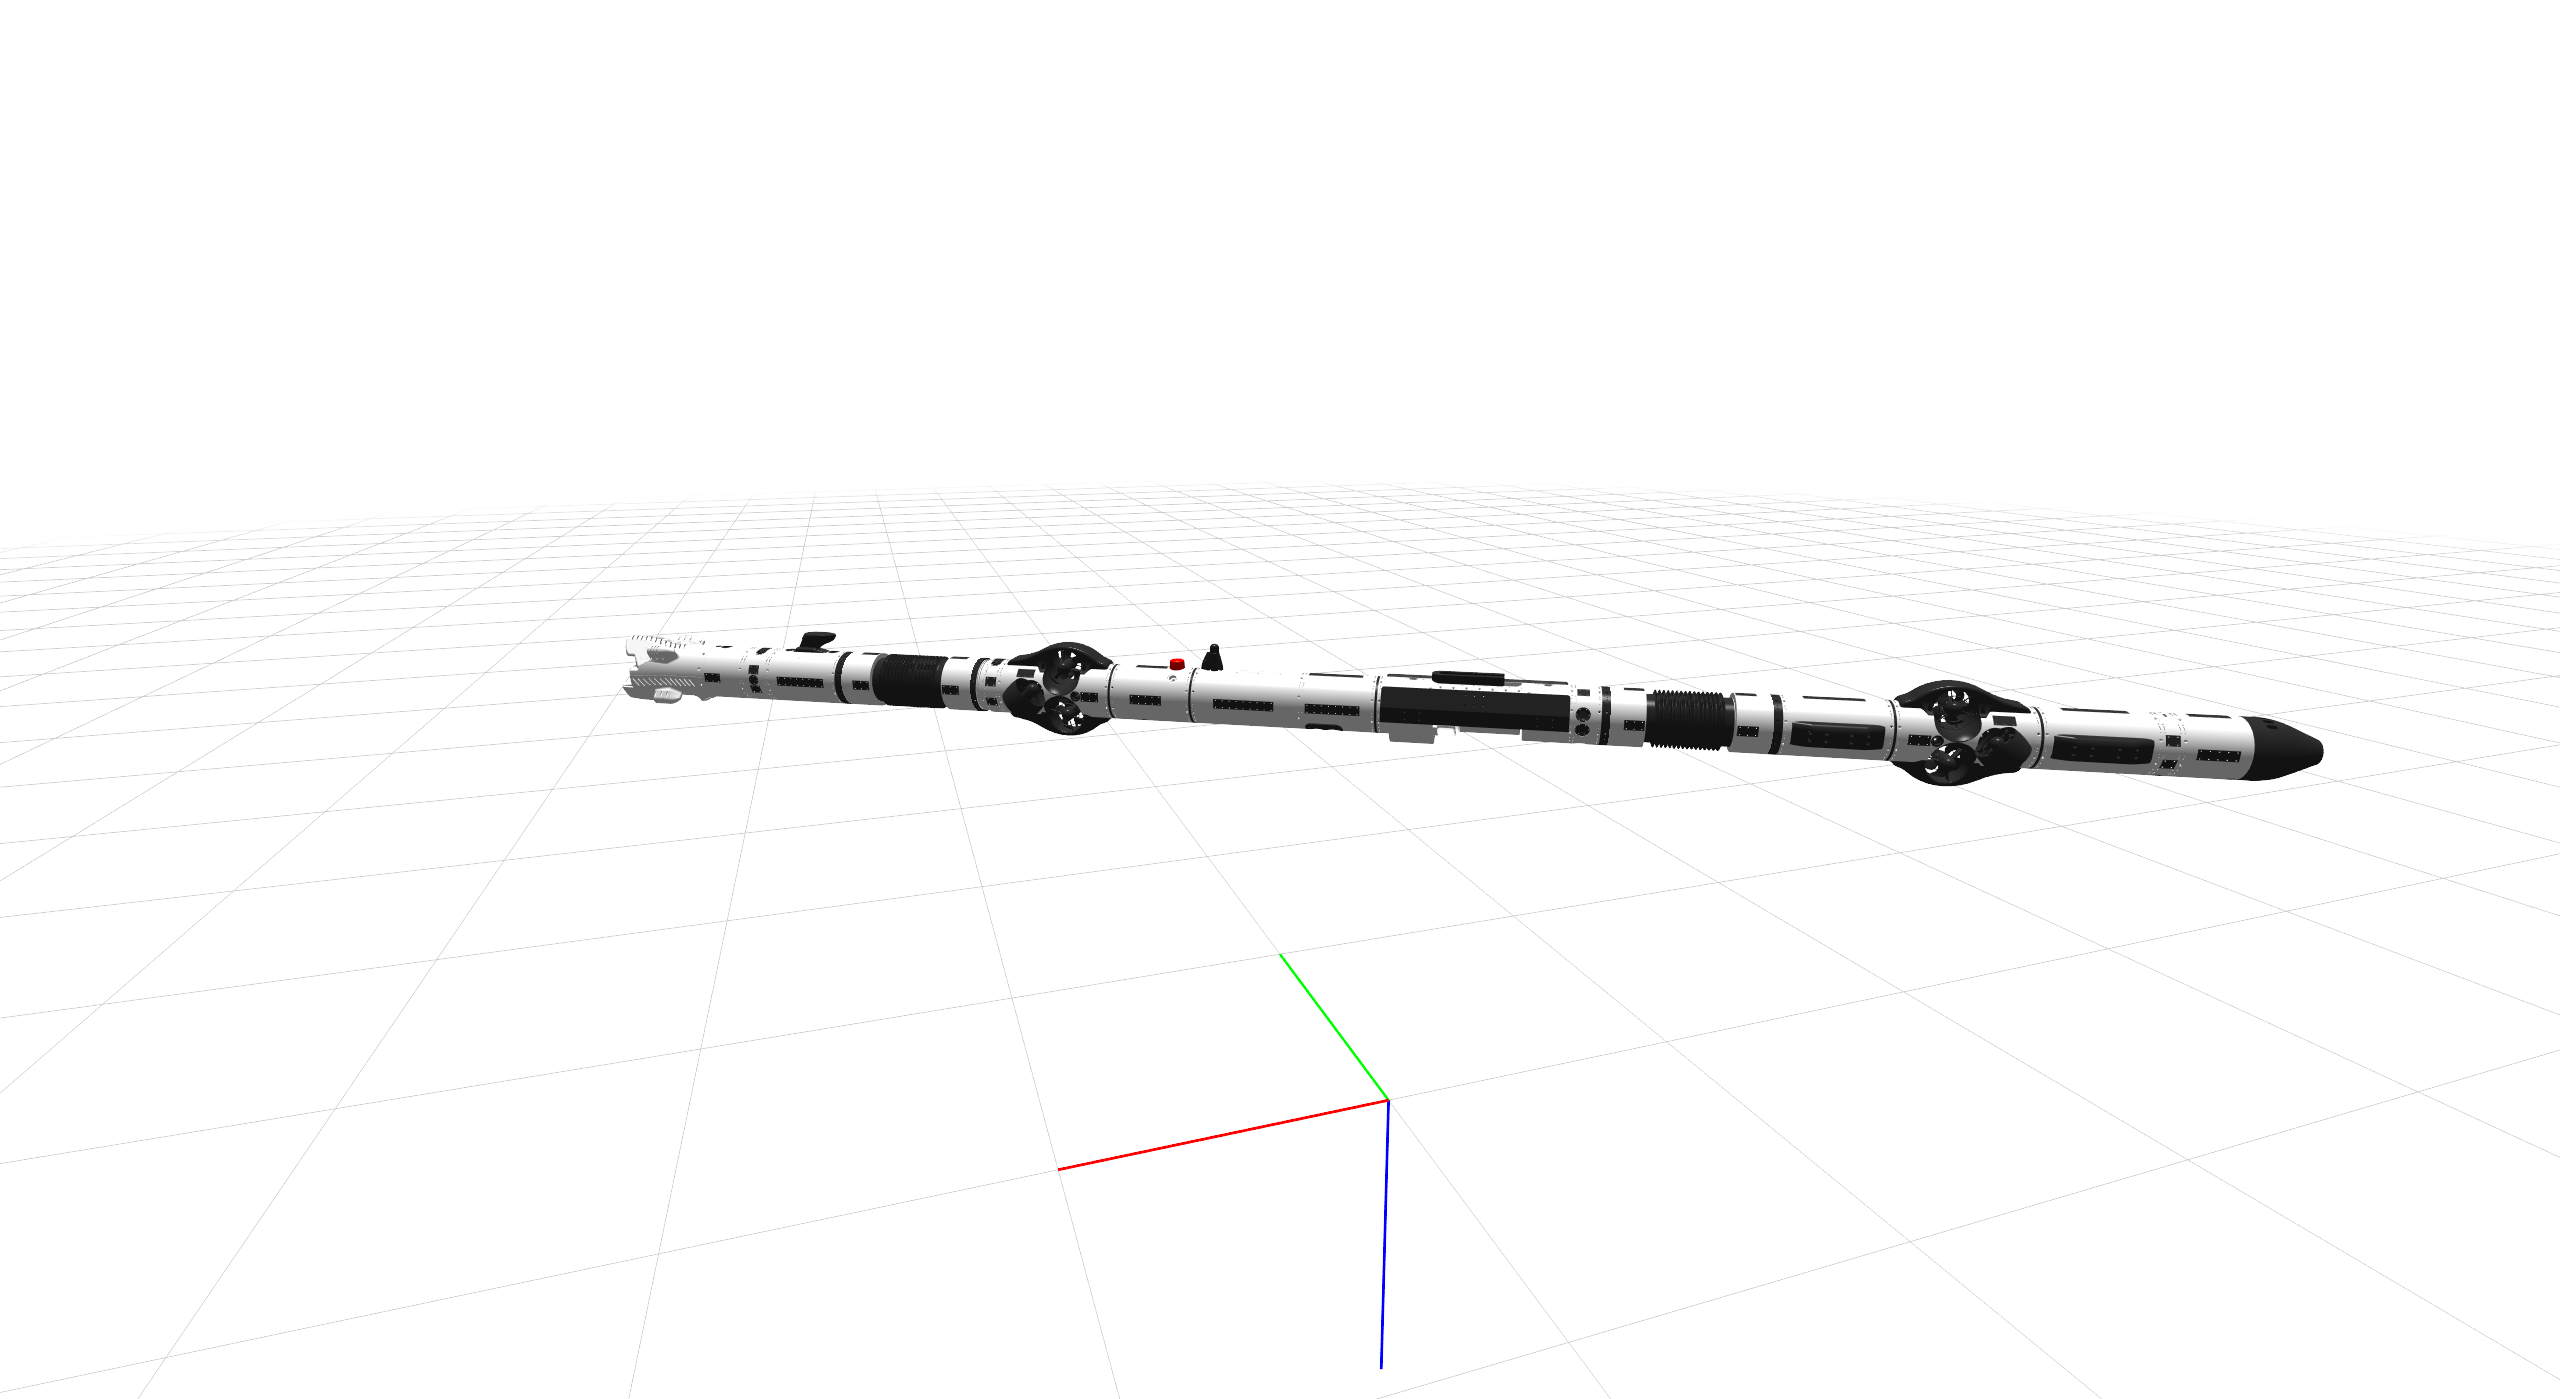
\includegraphics[width=\textwidth]{assets/eely-visualizer.png}
    \caption{A screenshot of the Eelume visualizer.}
    \label{fig:eelume:visualizer}
\end{figure}

% -----------------------------------------------------------------------------
\section{Assumptions and Limitations}
\label{sec:experimental_setup:assumptions_and_limitations}
In this section, key assumptions and limitations of the experimental setup are 
outlined to provide transparency and context for interpreting the results. 
These factors include both hardware and software constraints, as well as 
environmental conditions present during testing. While the control strategies 
are designed with general applicability in mind, practical aspects such as 
sensor noise, timing mismatches, and system-specific constraints may affect 
real-world performance. Identifying these limitations helps clarify the 
boundaries of the system's behavior and highlights areas for future 
improvement or calibration.

\subsection*{Control Loop Frequency}
Internally in the Eelume robot there is a data bus where messages are sent
between the different components of the robot. Messages setting references
to the indiviual thrusters and joint motors are sent on this bus. The bandwidth
limits on the bus puts constrains on how fast the controll loop can run. From
experiments, it was found that the bus can handle \(50\) Hz, but at higher
frequencies, degradations in performance were observed. The control loop is
therefore set to run at \(50\) Hz, being equivalent to a \(20\) ms loop time.
The continous-time controllers as presented in \autoref{ch:tpc} are called with
the latest measurements and references at this frequency, implicitly assuming
zero-order hold.
It is taught that the choosen loop time places minimal limtations on the performance
observed in the experiments as the frequency contents of the tasks are typically
very low, and underwater vehicles are typically not very fast systems. 

\subsection*{Encoder Jitter}
The Eelume robot is equipped with encoders on the joints which are used to measure the joint angles.
During experiments, it was observed that, sometimes, the joint angles jittered by up to \(10\) degrees,
giving false readings of the joint angles. From the visualization it is clear that this is not due to the robot moving,
as the the movement of the joints is smooth and continous. An example of the jitter is shown in \autoref{fig:eelume:encoder-jitter}.
\begin{figure}[h!]
    \centering
    \includegraphics[width=\textwidth]{assets/ignored/plots/jitter.pdf}
    \caption{An example of the encoder jitter observed during experiments.}
    \label{fig:eelume:encoder-jitter}
\end{figure}
The jittering seems to be more prominent for the first joint, although it is aboserved for all joints.
If this is the cause of some misconfiguration, broken encoders or some other issue is not known.
The high frequency contents in the joint measurements as a result of jittering
contributes to high frequency contents in the task-priority control signals. To
mitigate this, a first order low-pass filter is applied to the joint angles. The
low-pass filter is implemented in the control kit, and is applied to the joint angles before
they are used in the task-priority control framework. The low-pass filter can be
described by the following equation, where \(\alpha \in (0, 1)\) is the filter coefficient:
\begin{subequations}
\begin{align}
    \bm{\theta}_{\textrm{filtered}}[k] &= \alpha \bm{\theta}[k] + (1 - \alpha)\bm{\theta}_{\text{filtered}}[k-1] \\
    &= \bm{\theta}_{\textrm{filtered}}[k-1] + \alpha\left( \bm{\theta}[k] - \bm{\theta}_{\textrm{filtered}}[k-1] \right).
\end{align}
\end{subequations}
For the joint angles, the filter coefficient is set to \(\alpha = 0.39\). The
result of the low-pass filtering is shown in \autoref{fig:eelume:encoder-jitter-low-pass}.
We observe that the filtered joint angles closely follow the original angles,
and that some of the high frequency contents of the jitter is removed. Some discussion
about this method and alternative approaches are presented in \autoref{sec:conclusion:future_work}
\begin{figure}[h!]
    \centering
    \includegraphics[width=\textwidth,page=2]{assets/ignored/plots/jitter.pdf}
    \caption{Low-pass filtered joint angles to remove jitter.}
    \label{fig:eelume:encoder-jitter-low-pass}
\end{figure}

\subsection*{Topological Limitations}
As part of the aiding system for the \gls{ins}, the Eelume robot is equipped 
with a cNode transponder from Kongsberg for underwater acoustic positioning. 
This transponder communicates with a Kongsberg \(\mu\)-PAP acoustic positioning 
system, which provides periodic position corrections to the onboard \gls{ins}. 
The system achieves its highest accuracy when the transponder is positioned 
directly beneath the \(\mu\)-PAP.

In practice, however, the \(\mu\)-PAP is mounted on a crane at the harbor, while the 
Eelume robot is typically deployed about 10 meters away to allow space for 
experimentation. This offset results in a suboptimal angle between the \(\mu\)-PAP 
and the cNode transponder. To reduce the impact of this angle, the robot is 
positioned as deep as possible in the water—while still maintaining enough 
clearance for experiments—thereby minimizing the angle and improving 
positioning accuracy.

During experiments, forwarding from the acoustic positioning system is 
temporarily disabled for two main reasons. First, the system remains 
sufficiently accurate over the duration of the experiments. Second, when 
enabled, the system introduces periodic jumps in position data, which is 
disadvantagous when collecting data.

% -----------------------------------------------------------------------------
\subsection*{Velocity Measurement Noise}
The velocity measurements from the \gls{ins} were found to be noisy. Some measurements
from a typical run are shown in \autoref{fig:eelume:velocity-noise}. The linear
velocity of the \gls{aiauv} seems to be the smoothest, while there is some noise
on the angular velocity measurements. The noise is the most poromentent on
the angular velocity of the joints. From the figure one can se spikes reaching
velocities more than \(50\) degrees per second in absolute value, which is not realistic. Although the
reason for this noise is not known, it is likely related to the jitter on the 
joint measurements discussed in the previous sections, as the jitter seem to correlate in time
with the angular velocity spikes.

To mitigate the noise, a low-pass filter is applied to the velocity measurements.
The filter is first order, and is implemented in the control kit following the
same approach as for the joint angles. Because of the observed difference in
noise level between the linear, angular, and joint velocities, each of these
three components are filtered with different filter coefficients. The coefficients
are presented in \autoref{tab:eelume:vel-filters}.

%0.334511
%0.273779
%0.0245166
\begin{table}[h]
    \centering
    \begin{tabular}{|c|c|}
        \hline
        Velocity Component & Filter Coefficient \(\alpha\) \\ \hline \hline
        Linear Velocity & \(0.33\) \\ \hline
        Angular Velocity & \(0.27\) \\ \hline
        Joint Velocity & \(0.025\) \\ \hline
        \hline
    \end{tabular}
    \caption{Filter coefficients for the low-pass filtering of velocity measurements.}
    \label{tab:eelume:vel-filters}
\end{table}

The result of the low-pass filtering is shown in \autoref{fig:eelume:velocity-noise-low-pass}.
The low-pass filtered velocities are much smoother, and the spikes in the angular
velocities are removed to a large extent. A side-by-side comparison of the unfiltered
and low-pass filtered velocities is shown in \autoref{fig:eelume:velocity-noise-low-pass-comp}.
From this figure, it is clear that much of the high-frequency contents in the velocity measurements
is removed without causing significant delay in the measurements. The advantages and disadvantages
of using a low-pass filter on the velocity measurements are discussed in more detail in \autoref{sec:results:lowpass_filtering}.

\begin{figure}[h!]
    \centering
    \includegraphics[width=\textwidth,page=1]{assets/ignored/plots/velnoise.pdf}
    \caption{Unfiltered velocity measurements from the \gls{ins} during experiments.}
    \label{fig:eelume:velocity-noise}
\end{figure}

\begin{figure}[h!]
    \centering
    \includegraphics[width=\textwidth,page=2]{assets/ignored/plots/velnoise.pdf}
    \caption{Low-pass filtered velocity measurements.}
    \label{fig:eelume:velocity-noise-low-pass}
\end{figure}

\begin{figure}[h!]
    \centering
    \includegraphics[width=\textwidth,page=3]{assets/ignored/plots/velnoise.pdf}
    \caption{Comparison of unfiltered and low-pass filtered velocity measurements.}
    \label{fig:eelume:velocity-noise-low-pass-comp}
\end{figure}

% -----------------------------------------------------------------------------
\subsection*{\gls{ins} Limitations}
The Sunstone \gls{ins} used in the Eelume robot offers several configuration options that can impact experimental performance. One key feature is a roll rate limitation: if the \gls{ins} detects that the roll rate exceeds a certain threshold, it assumes the measurements are unreliable and disables control inputs. This is a built-in safety mechanism, which makes sense during normal operation when rapid rolling is not expected. However, this limitation is not particularly problematic in this context, as the experimental tasks are designed to be relatively low-frequency and thus naturally avoid high roll rates. It is mentioned here as an important consideration during testing, since avoiding large roll rates can prevent unnecessary interruptions and time-consuming recalibrations.

A crucial component of the \gls{ins} is the \gls{dvl}, which measures the robot’s velocity relative to the sea floor. Due to the mounting orientation of the \gls{dvl}, large roll or pitch angles can reduce its accuracy, a condition commonly referred to as losing \textit{bottom lock}. Without bottom lock, the \gls{ins} becomes significantly less reliable. To maintain bottom lock during experiments, the robot is kept at low roll and pitch angles, and large vertical movements are avoided.

\subsection*{Wave Influence and Water Salinity}
The experiments were conducted at \gls{tbs}, located in the fjord just outside 
Trondheim, Norway. Wave influence was observed to vary depending on weather 
conditions, particularly when winds came from the north or northeast, 
resulting in more pronounced surface motion. To minimize this disturbance, 
experiments were scheduled during calm weather with minimal wave activity.

Water salinity was also found to vary with weather, affecting the robot's 
buoyancy. Specifically, the depth at which the Eelume robot passively 
stabilizes—without using its thrusters—changed from day to day. This variation 
is important to account for, as the hydrostatic forces are compensated for in 
the \gls{pd+} controller. To reduce the impact of salinity changes, tests were 
carried out at depths where the water column exhibited relatively stable 
salinity levels.

\subsection*{Lower-Level Thruster and Joint Motor Control}
The Eelume \gls{api} provides a way to set thruster force references and joint
torque references. However, it is not known how well these references are
followed by the thrusters and joint motors. This is information that is simply
not available in the \gls{api}, and can therefore not be used in the controller.
For the sake of simplicity, it is assumed that the thrusters and joint motors
follow their references up to the frequency contents of the control inputs.

The joint motors are also limited to give a maximum torque of \(16\) Nm. To take
this into account, the joint controllers need to be tuned to ensure that the
joint torques do not exceed this limit by a large margin. The thrusters are set
to have a wattage limit of \(125\) W each, ensuring that the Eelume robot does
not experience a brownout during experiments. The wattage limit is set using the
\gls{api} and is not a hard limit, but was chosen for safety reasons.

% -----------------------------------------------------------------------------
\section{Experimental Procedures}
\subsection*{Launch and test procedures}
\begin{itemize}
    \item Launch and test procedures
    \item show the response of the lower-level DP+ controller.
    \item Head + Tail stretching out
    \item Bending with joint constraints
    \item Expected results?
\end{itemize}

